%%%%%%%%%%%%%%%%%%%%%%%%%%%%%%%%%%%%%%%%%
% Short Sectioned Assignment
% LaTeX Template
% Version 1.0 (5/5/12)
%
% This template has been downloaded from:
% http://www.LaTeXTemplates.com
%
% Original author:
% Frits Wenneker (http://www.howtotex.com)
%
% License:
% CC BY-NC-SA 3.0 (http://creativecommons.org/licenses/by-nc-sa/3.0/)
%
%%%%%%%%%%%%%%%%%%%%%%%%%%%%%%%%%%%%%%%%%

%----------------------------------------------------------------------------------------
%	PACKAGES AND OTHER DOCUMENT CONFIGURATIONS
%----------------------------------------------------------------------------------------

\documentclass[paper=a4, fontsize=11pt]{scrartcl} % A4 paper and 11pt font size
\usepackage{xeCJK}
\usepackage{fourier} % Use the Adobe Utopia font for the document - comment this line to return to the LaTeX default
\usepackage[T1]{fontenc} % Use 8-bit encoding that has 256 glyphs
\usepackage[english]{babel} % English language/hyphenation
\usepackage{amsmath,amsfonts,amsthm} % Math packages
\usepackage{titlesec}
\usepackage{titletoc}
\usepackage{abstract}
\usepackage[toc,page,title,titletoc,header]{appendix}
\usepackage{lipsum} % Used for inserting dummy 'Lorem ipsum' text into the template

\usepackage{sectsty} % Allows customizing section commands
\allsectionsfont{\normalfont\scshape} % Make all sections centered, the default font and small caps

\usepackage{fancyhdr} % Custom headers and footers
\pagestyle{fancyplain} % Makes all pages in the document conform to the custom headers and footers
\fancyhead{} % No page header - if you want one, create it in the same way as the footers below
\fancyfoot[L]{} % Empty left footer
\fancyfoot[C]{} % Empty center footer
\fancyfoot[R]{\thepage} % Page numbering for right footer
\renewcommand{\headrulewidth}{0pt} % Remove header underlines
\renewcommand{\footrulewidth}{0pt} % Remove footer underlines
\setlength{\headheight}{13.6pt} % Customize the height of the header

\numberwithin{equation}{section} % Number equations within sections (i.e. 1.1, 1.2, 2.1, 2.2 instead of 1, 2, 3, 4)
\numberwithin{figure}{section} % Number figures within sections (i.e. 1.1, 1.2, 2.1, 2.2 instead of 1, 2, 3, 4)
\numberwithin{table}{section} % Number tables within sections (i.e. 1.1, 1.2, 2.1, 2.2 instead of 1, 2, 3, 4)

\setlength\parindent{0pt} % Removes all indentation from paragraphs - comment this line for an assignment with lots of text
\bibliographystyle{plain}

\usepackage[colorlinks,linkcolor=black,anchorcolor=blue,citecolor=green, urlcolor = blue]{hyperref} % Using hyper reference
\usepackage{multirow}
\usepackage{geometry}
\usepackage{setspace}

%-------------------------------------------------------------------
%	CONTENT SECTION
%-------------------------------------------------------------------
\usepackage[nottoc]{tocbibind}
%\titlecontents{section}
%	[0 em]
%	{\filcenter\large\scshape}
%	{}
%	{}
%	{\titlerule*[1em]{$\cdot$}\contentspage}
%

%-------------------------------------------------------------------
%	TITLE SECTION
%-------------------------------------------------------------------
\newcommand{\horrule}[1]{\rule{\linewidth}{#1}} % Create horizontal rule command with 1 argument of height

\title{	
\normalfont \normalsize 
\textsc{Zhiyuan College, Shanghai Jiao Tong University} \\ % Your university, school and/or department name(s)
\horrule{0.5pt} \\[0.4cm] % Thin top horizontal rule
\huge Five-Stage MIPS Pipeline in Verilog HDL \\ % The assignment title
\horrule{2pt} \\ % Thick bottom horizontal rule
}

\author{
\normalsize
	Yurong You (ID: 5140519064)\\
\normalsize
	ACM Honored Class
} % Your name

\date{\normalsize\today} % Today's date or a custom date

\begin{document}
\maketitle % Print the title
\begin{spacing}{1.5}
\renewcommand{\abstractname}{\scshape \bfseries \large Abstract}
\begin{abstract}
	This report is a detailed summary on the five-stage MIPS pipeline project I have finish in this summer. The design is elaborated on both the whole and the part in this report. The pipeline supports all MIPS standard integer instructions except those related to coprocessors, and the forwarding, hazard control and branch control techniques are all fully implemented. The pipeline not only passes the basic Yamin Li's experiment code, but passes all self-designed test cases which are intended to test the pipeline's completeness on supporting every part of the MIPS integer instruction set. Source code in Verilog HDL and the pipeline blueprint are also provided.
\end{abstract}
\newpage
\renewcommand{\contentsname}{\scshape \bfseries \Large Contents}
\tableofcontents

\newpage
\section{Introduction and Design Philosophy}
	This report is for the final project of course MS108, computer system I. In this project, I implemented a comprehensive MIPS classical five-stage pipeline which supports all but two (coprocessor instructions) MIPS standard integer instructions\footnote{\url{https://en.wikipedia.org/wiki/MIPS_instruction_set}}. A summary on the supported instruction set are presented in appendix \ref{app::inst}.
	
	On designing the structure of pipeline, I take \cite{lsl} and \cite{lym} as reference, but I found that different functional units in Lei's design are coupling with each other, which will lead to inconvenience if we are to extend the functionality of our pipeline, and a large part of Li's design are low-level implementations on function units, which I think might be unnecessary. Thus I decided to design a pipeline for myself, follows the following principles,
	
	\begin{spacing}{1.0}
	\begin{enumerate}
		\item Register-Transfer Level (RTL) modelling;
		\item Separate different stages;
		\item Separate control-path and data-path.
	\end{enumerate}
	\end{spacing}
	
	The blueprint of my design is presented in appendix \ref{app::blueprint}, note that due to the limited space, I do not circle what stage module consists of what sub-modules.
	
	The branch control, hazard control and forwarding are inspired by \cite{COD}. Different functional units are implemented in different modules, the main part of which will be introduced in the next section. The modules are connected by \verb|pipeline.v| to compose the whole pipeline.
	
	Source code is available on \url{https://github.com/YurongYou/MIPS_CPU} (will be set public after project deadline).
\newpage
\section{Main Modules Elaboration}
    \subsection{Stage Modules}
    	There are five stages in this five-stage MIPS pipeline.
    	\subsubsection{Instruction Fetch} Implemented in \verb|IF.v|. The main function of this module is to generate \verb|PC|, the address of current instruction, which will be sent to instruction memory (\verb|ROM|) in \verb|pipeline.v| to access instruction. This module consists of merely a D-type flip-flop with enable port to store the address. It takes control signals and branch address from hazard control module and branch control module to implement those control.
    	\subsubsection{Instruction Decode} Implemented in \verb|ID.v|. This module is mainly a decoder, which takes instruction from IF module as the input and outputs several control signals. Those signals are
    		\begin{table}[!htb]
				\centering
				\begin{tabular}{|l|l|}
				\hline
				\multicolumn{1}{|c|}{Signal} & \multicolumn{1}{c|}{Meaning}                                    \\ \hline
				WriteReg                     & whether or not is to write register                             \\ \hline
				MemOrAlu                     & the source to write register is from memory or ALU              \\ \hline
				WriteMem                     & whether or not is to write memory                               \\ \hline
				ReadMem                      & whether or not is to read register                              \\ \hline
				AluType                      & the type of computation to perform in ALU in execution stage    \\ \hline
				AluOp                        & the subtype of computation to perform in ALU in execution stage \\ \hline
				AluSrcA                      & the first source of ALU is (rs or shamt)                        \\ \hline
				AluSrcB                      & the second source of ALU is (immediate or rt)                   \\ \hline
				RegDes                       & which register is to be write                                   \\ \hline
				ImmSigned                    & use signed or unsigned extended immediate                       \\ \hline
				is\_jal                      & whether or not this instruction is a jal instruction            \\ \hline
				\end{tabular}
				\caption{A Summary on the decoder's output signals}
			\end{table}
			
			Note that the ``MemOrAlu'' signal is indeed redundant (can be inferred from ``WriteReg''); and the reason why there should be a ``is\_jal'' signal is that this instruction is asking to put $\mathrm{PC}+4$ into the $31$th register and jump to a specific instruction address, which is too special to be integrated effortlessly with other instructions in my implementation. These signal will go all the way down to the following stage to control the pipeline. 
			
			This module also output several (signed/unsigned extended) segmentations on the instruction such as shamt, imm, etc.
    	\subsubsection{Execution} Implemented in \verb|EX.v|. This module implements the forwarding on the source of ALU and performs the computation specified by ``AluType'' and ``AluOp'' in ALU. The forwarding is performed according to the signals sent by the forwarding module.
    	\subsubsection{Memory Access} Implemented in \verb|MEM.v|. Memory access follows the standard of Wishbone Bus  \footnote{\url{https://en.wikipedia.org/wiki/Wishbone_(computer_bus)}}, which has a brief usage guide on page 257 of book \cite{lsl}. I use a write memory controller and a read memory control to modify the data in order to get the desired form. This module also implements the forwarding on the source of memory write according to the signals sent by the forwarding module.
    	
    	\subsubsection{Write Back} Not implemented as a single module, since there is just one switch on the source of data, from the ALU or the memory, to write back into the register file.

    \subsection{Stage Sandwich Modules}
    	Also called ``pipeline registers'', but I prefer this name. These modules are merely collections of D-type flip-flops with enable port, which can update data on the rising edge of clock. See source code \verb|if_id.v|, \verb|id_ex.v| and \verb|ex_mem.v|.
    \subsection{Control Modules}
    	\subsubsection{Forwarding}
	    	 Forwarding unit takes signals from various stages and output the forwarding control signals. There are 7 kinds of forwarding, and the control logic is presented as follows,
	    	 \begin{enumerate}
	    	 	\item Forward Alu result in MEM stage to EX stage
	    	 	
	    	 	\verb|data_addr_EX == target_MEM && WriteReg_MEM == `WriteEnable &&| \\
	    	 	\verb|target_MEM != 0|
	    	 	
	    	 	\item Forward Alu result in WB stage to EX stage
	    	 	
	    	 	\verb|data_addr_EX == target_WB && WriteReg_WB == `WriteEnable &&| \\
	    	 	\verb|target_WB != 0|
	    	 	
	    	 	\item Forward Mem result in WB stage to MEM stage (A load followed by a store)
	    	 	
	    	 	\verb|data_addr_MEM == target_WB && WriteReg_WB == `WriteEnable &&| \\
	    	 	\verb|target_WB != 0|
	    	 	
	    	 	\item Forward Alu result in EX stage to ID stage (for branch control)
	    	 	
	    	 	\verb|data_addr_ID == target_EX && WriteReg_EX == `WriteEnable &&| \\
	    	 	\verb|target_EX != 0|
	    	 	
	    	 	\item Forward Alu result in MEM stage to ID stage (for branch control)
	    	 	
	    	 	\verb|data_addr_ID == target_MEM && WriteReg_MEM == `WriteEnable &&| \\
	    	 	\verb|target_MEM != 0|
	    	 	
	    	 	\item Forward Hi/Lo in MEM stage to EX stage
	    	 	
	    	 	\verb|we_hi(lo)_MEM == `WriteEnable|
	    	 	
	    	 	\item Forward Hi/Lo in WB stage to EX stage

	    	 	\verb|we_hi(lo)_WB == `WriteEnable|
	    	 	
	    	 \end{enumerate}
    	\subsubsection{Hazard Control}
    		There will be only one kind of hazard in my implementation: a load instruction immediately followed by an not-store operation which has data dependency on it. In this case, we need to stall the pipeline for one cycle --- keep PC register and IF/ID sandwich register remain unchanged and reset ID/EX sandwich register to zero in the next clock cycle.
    	\subsubsection{Branch Control}
    		Branch control can be viewed as performed in the ID stage. Since in my implementation there is no delay slot, we have to abandon the previous fetched instruction in IF stage if branch is taken. In practice, just reset the If/ID sandwich register in the next clock cycle and sent the branch address to the PC register.
    \subsection{Register File}
    	Note that the register file writes at the falling edge. The reason of doing so is that if the register writes at the rising edge, the same with sandwich register, it will write the data in the next clock cycle, which leads to some additional code to support forwarding inside register file. 
\section{Test Summary}
	All test code is available on \url{https://github.com/YurongYou/MIPS-CPU-Test-Cases}. There are 8 tests in total, 6 of them are respectively intended to test a major part of the MIPS integer instructions. And there is a Li's experiment code test. On each test folder, there are instruction data (\verb|.data|), MIPS source code (\verb|.s|) and my waveform simulation screenshot (\verb|.png|). The waveform is captured on Scansion\footnote{\url{http://www.logicpoet.com/scansion/}}.
	
	To run the tests,
	\begin{enumerate}
		\item modify the \verb|SOPC.v| file, include the pipeline, fill in the corresponding instruction data location;
		\item compile the \verb|SOPC.v| (I use iverlog\footnote{\url{http://iverilog.icarus.com}} on mac).
		\item observe the waveform, take branch test as example in figure \ref{fig::branch}
		\begin{figure}[!htb]
			\centering
			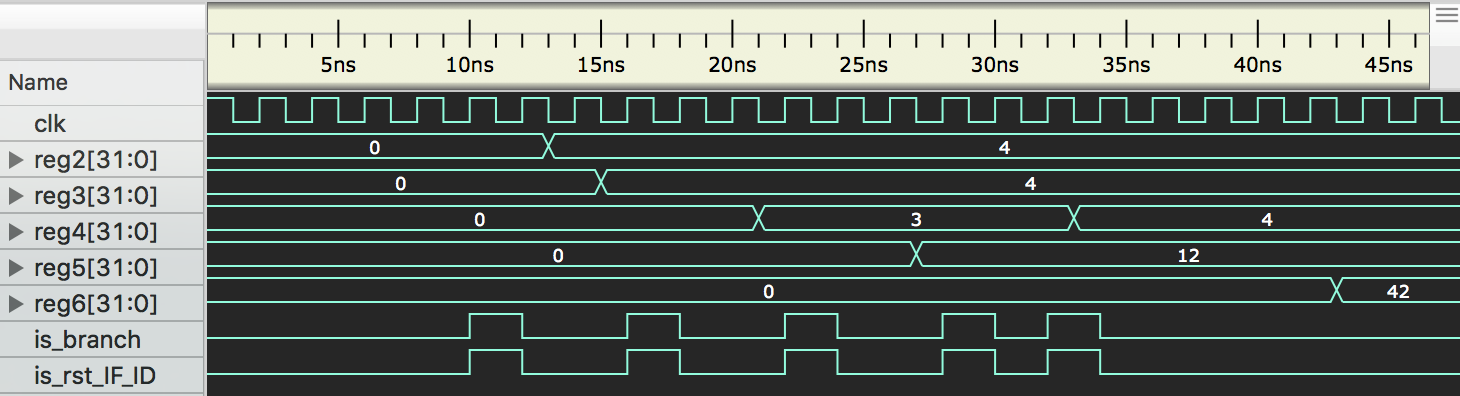
\includegraphics[width = 13 cm]{branch}
			\caption{waveform for branch test}
			\label{fig::branch}
		\end{figure}
		
		It is easy to check that the pipeline is running as expected, which finally writes the answer to life, the universe and everything into register 6.
	\end{enumerate}
\section{Further Enhancement}
	\begin{enumerate}
		\item Out of order execution. I think classical five-stage pipeline is quite difficult to improve performance. Straight forward ways to speed up such as multiple issue and multiple ALUs will be hard to be implemented under in-order execution pipeline structure. Thus maybe dynamic scheduling structure will have better promise on the performance.
		\item Cache. I have not implement cache by now since all test is functional simulation and there is no memory delay. If we are to run the pipeline on the FPGA using the provided RAM, data cache and instruction cache are indispensable.
		\item Exception and interrupt. To run an operation system, the CPU must be able to handle internal exception such as overflow, system call, etc. and external interrupt such as I/O.
		\item Synthesis on FPGA. This is the ultimate goal of the project, but there still a lot to tackle on it.
	\end{enumerate}
	\section{Acknowledgement}
	Special thanks to Zihao Ye, Zhijian Liu and Tianyao Chen for effective discussion.
\newpage
\nocite{*}
\bibliography{cpu}

\newpage
\renewcommand{\appendixpagename}{\scshape \Large \mdseries \rmfamily Appendices}
	\newgeometry{bottom = 1.3 cm }
\begin{appendices}
    \renewcommand{\thesection}{\Alph{section}}
    
    \section{Instruction Summary}
    	\label{app::inst}
    	\begin{table}[!htb]
    		\centering
    		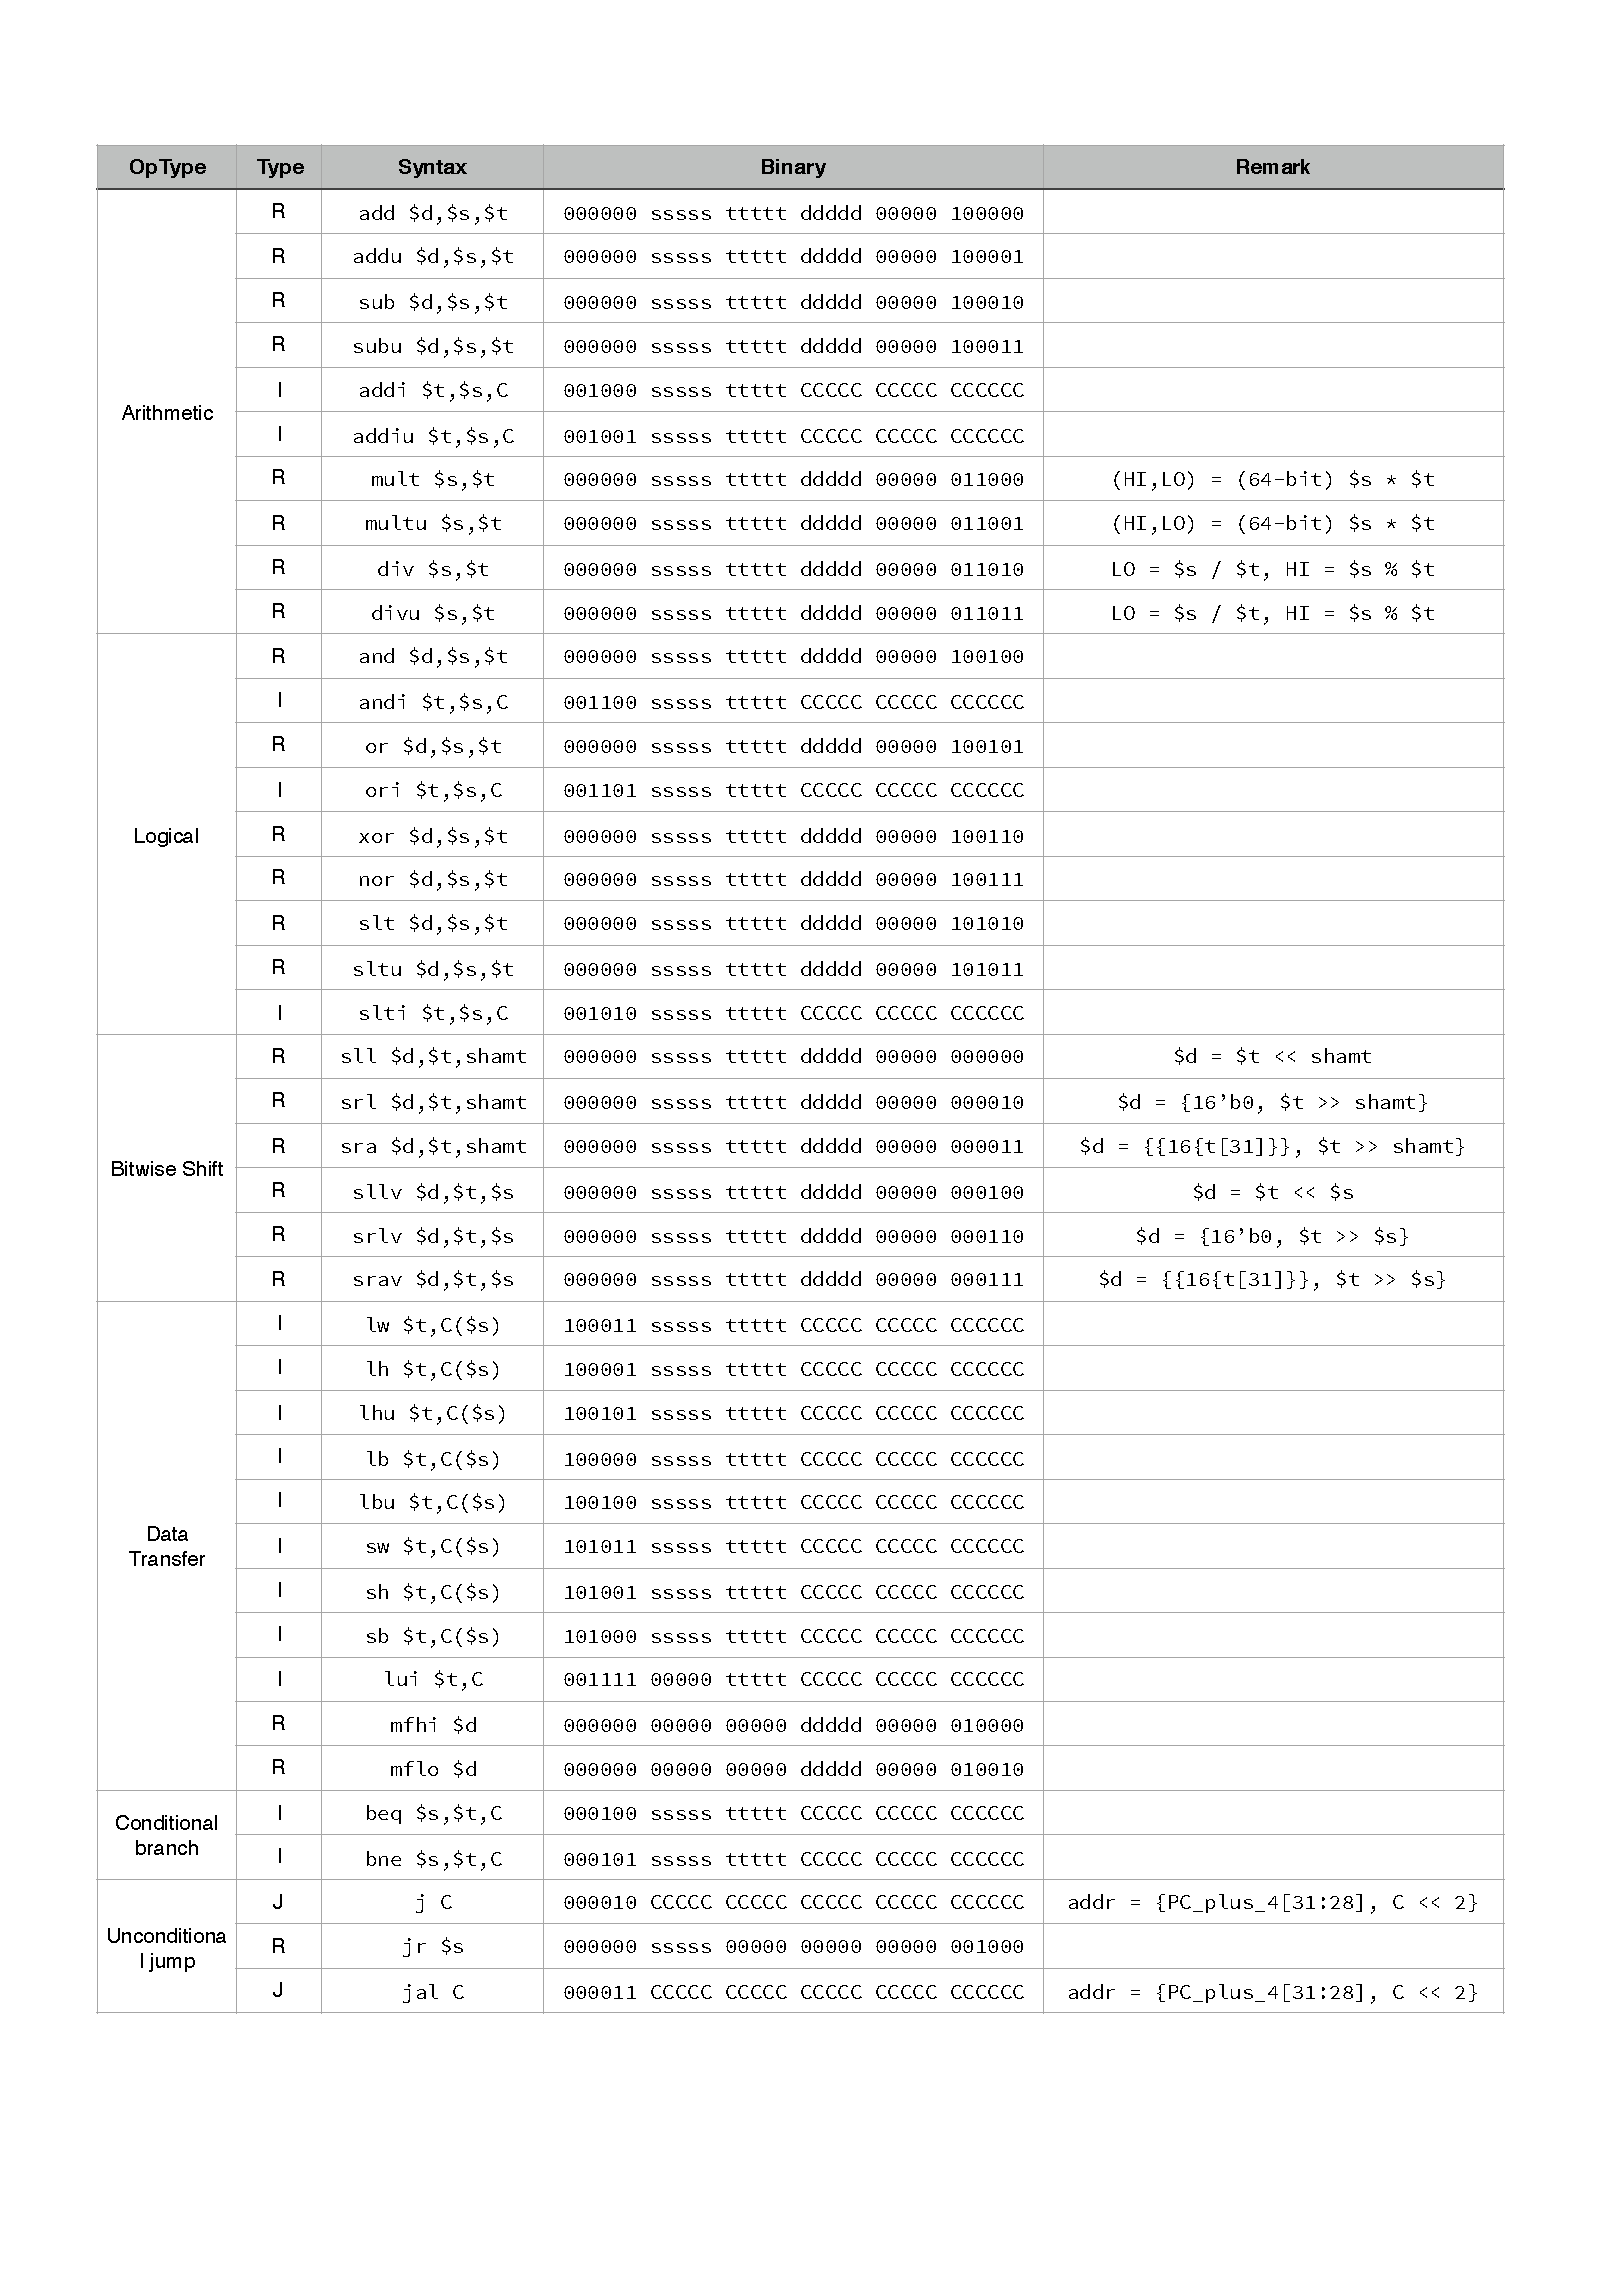
\includegraphics[width = 14cm]{Instructions}
    		\caption{A summary on supported MIPS instructions}
    	\end{table}
    \newpage
    \section{Pipeline Blueprint}
    	\label{app::blueprint}
	    \begin{figure}[!htb]
	    	\centering
	    	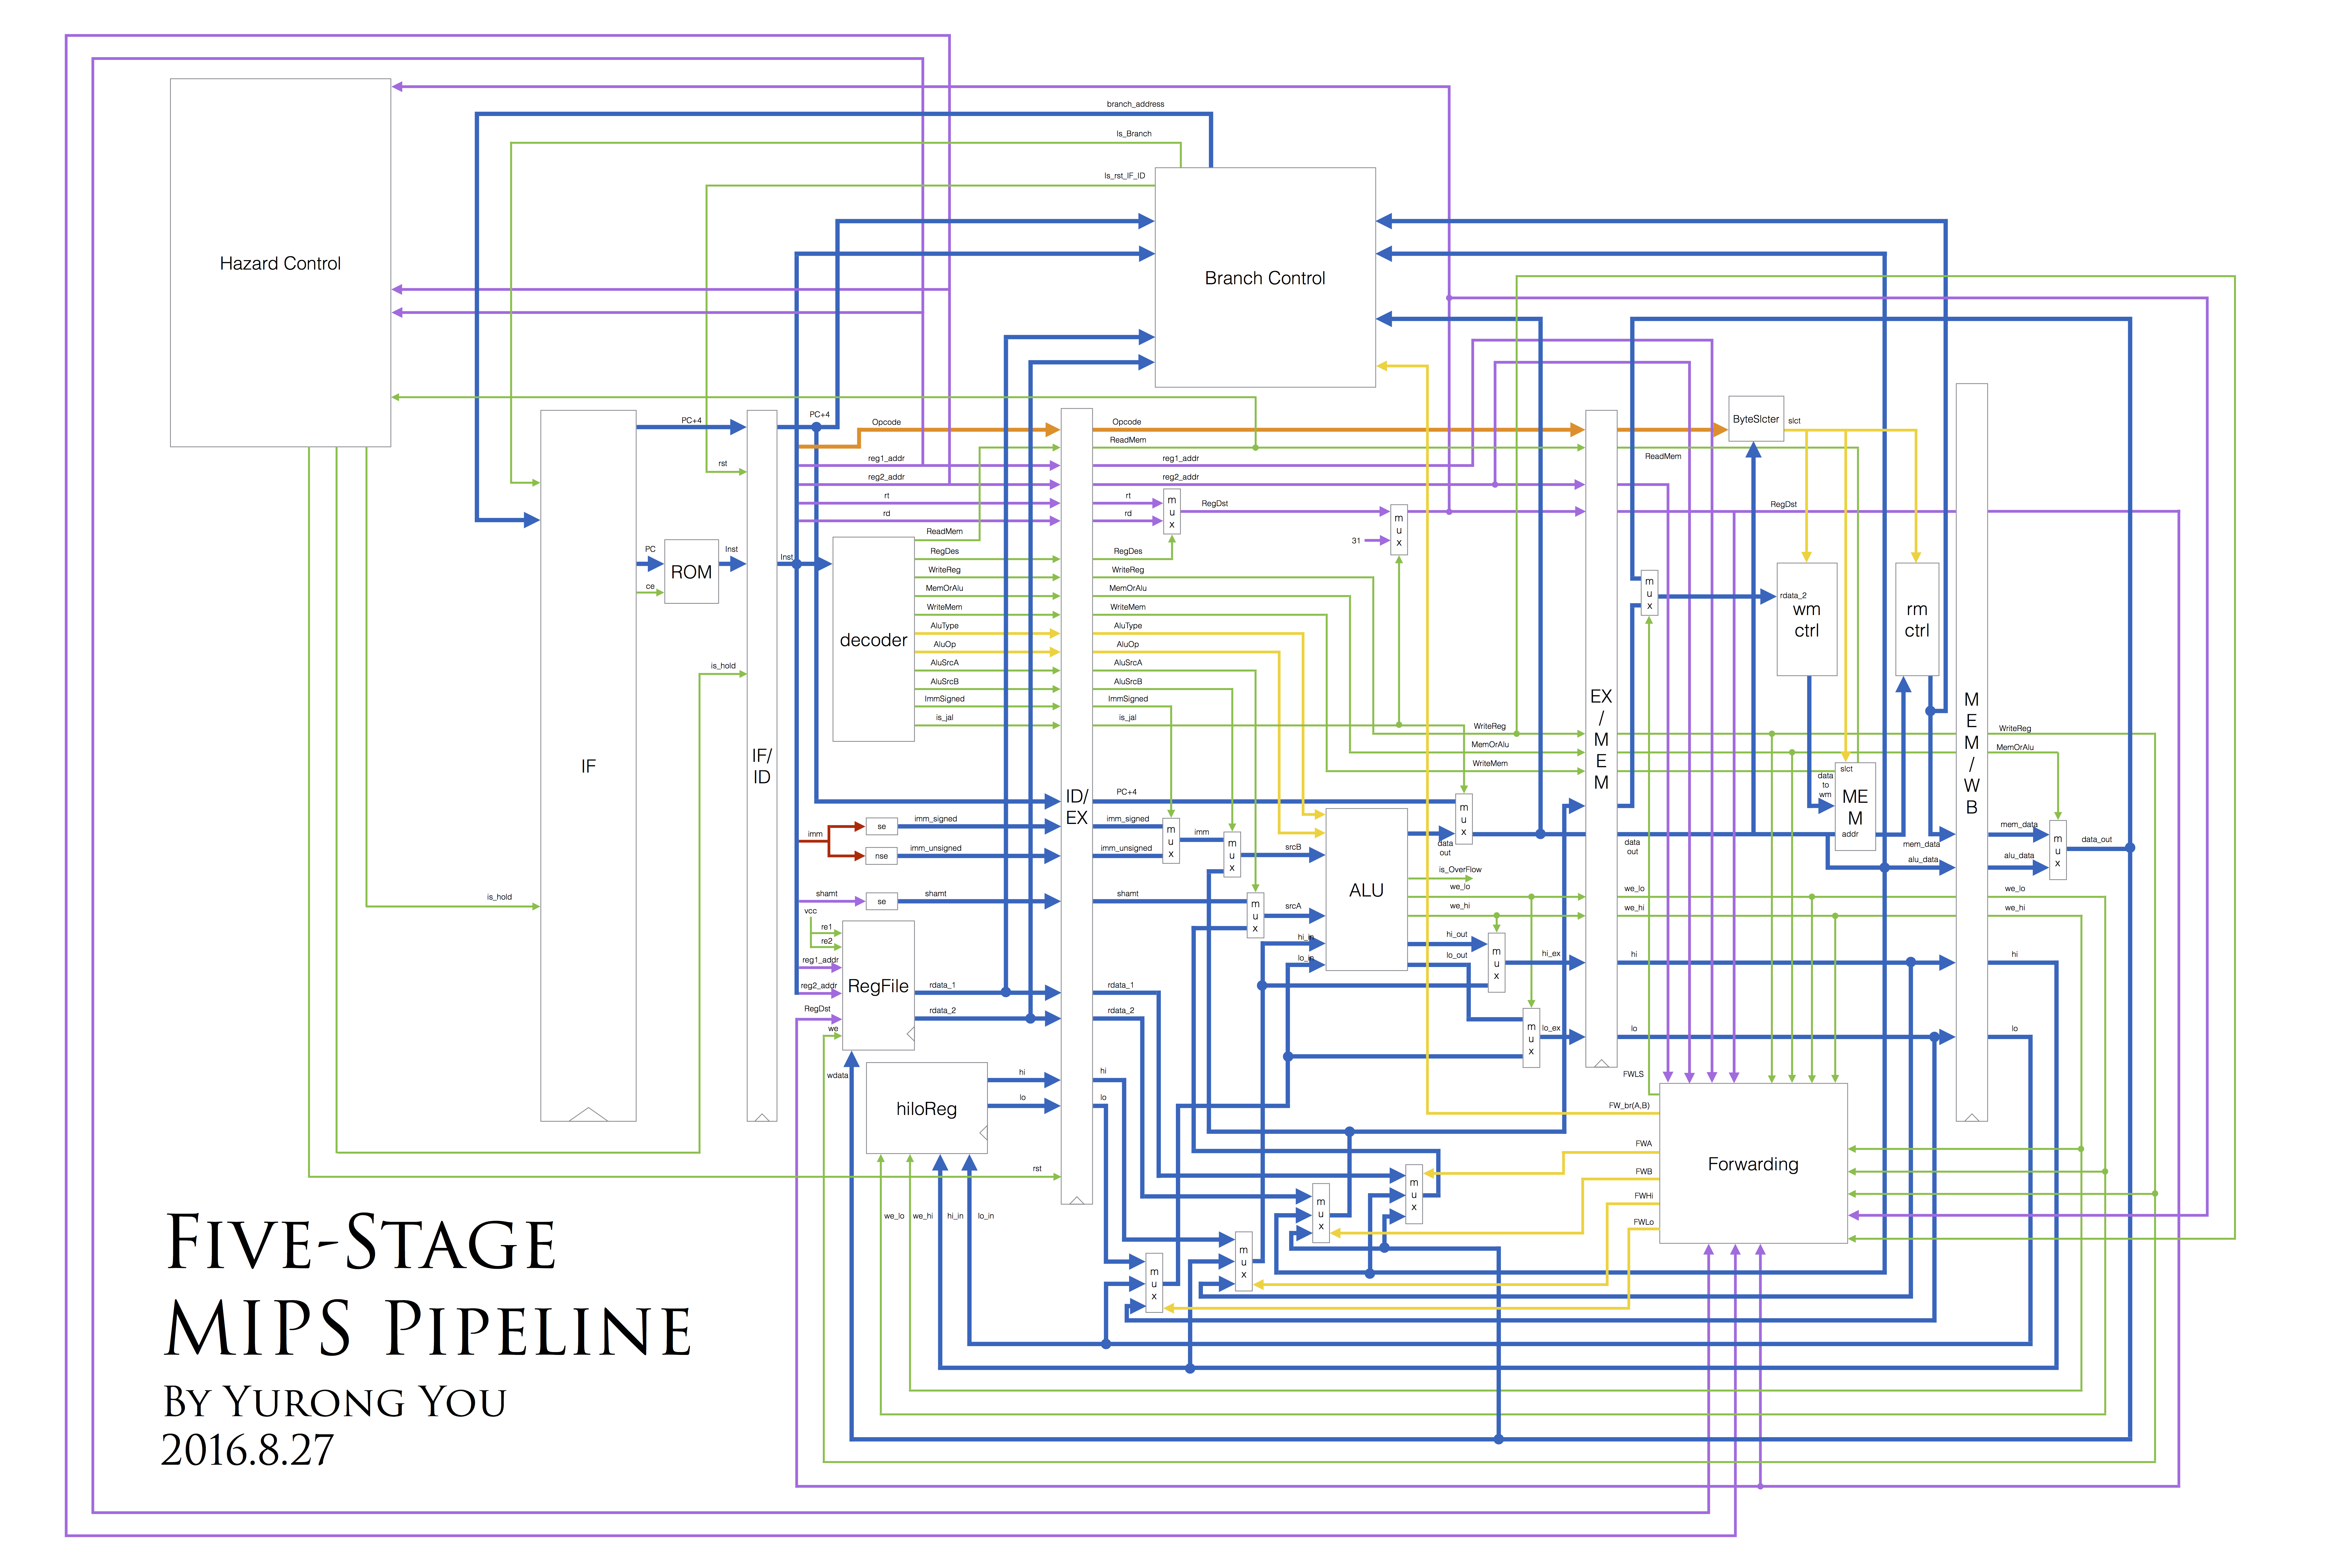
\includegraphics[angle=90,origin=c, width = 15cm]{blueprint}	    	
	    \end{figure}
\end{appendices}
\end{spacing}
\end{document}